%File: formatting-instruction.tex
\documentclass[letterpaper]{article} %DO NOT CHANGE THIS
\usepackage{aaai19}  %Required
\usepackage{times}  %Required
\usepackage{helvet}  %Required
\usepackage{courier}  %Required
\usepackage{url}  %Required
\usepackage{graphicx}  %Required
\usepackage{amsmath}
\usepackage{mathrsfs}
\usepackage{color,soul}
\usepackage{listings}
\usepackage{caption,subcaption}
\usepackage{natbib}


\newcounter{tmp}

% \usepackage{fontspec}
% \usepackage{unicode-math}

% new command
% \newcommand{\stripsp}{{\sc strips+}}
\newcommand{\stripsp}{{strips+}}
% \newcommand{\pddlthree}{{\sc PDDL3}}
\newcommand{\pddlthree}{{PDDL3}}
\newcommand{{\lama}}{{{LAMA}}}
\newcommand{\mercury}{{Mercury}}
\newcommand{{\fdss}}{{Fast Downward Stone Soup 2018}}
\newcommand{{\fdssshort}}{{FDSS 2018}}

\newcommand{{\miplan}}{{MIPlan}}
\newcommand{{\ibacop}}{{IBaCoP2}}
\newcommand{{\fdremixcomplete}}{{Fast Downward Remix}}
\newcommand{\lprpgp}{{LPRPG-P}}
\newcommand{{\fdremix}}{{FD-Remix}}
% \newcommand{{\fifthIPC}}{{{IPC5}}}


\frenchspacing  %Required
\setlength{\pdfpagewidth}{8.5in}  %Required
\setlength{\pdfpageheight}{11in}  %Required
%PDF Info Is Required:
  \pdfinfo{
/Title (Compiling PDDL3 Qualitative Preferences without Using Automata)
/Author (Anonymous)}
\setcounter{secnumdepth}{0}  
 \begin{document}
% The file aaai.sty is the style file for AAAI Press 
% proceedings, working notes, and technical reports.
%
\title{Compiling PDDL3 Qualitative Preferences without Using Automata}
\author{...
}
\maketitle
\begin{abstract}
...
\end{abstract}

\section{Introduction}
\section{Related Work}
\section{Propositional Planning with Qualitative PDDL3 Preferences}
\section{Operator-Preference Interactions}
\section{Compilation of Qualitative Preferences}
\section{Experimental Results}







\subsection{Experiments Description}
We implemented the proposed compilation scheme and have evaluated it
by two sets of experiments with different purposes. On the one hand we
evaluated the scheme in a satisficing planning context in which we focused
on the search for sub-optimal plans, while in the other we focuse on the
search of optmial plans.

Regarding the comparison in the context of the satisficing planning
we have considered the following {\stripsp} planning system
{\lama}\cite{RicLAMA}, {\mercury} \cite{MercuryIPC8},
{\miplan} \cite{nunez2014miplan}, {\ibacop} \cite{cenamor2014ibacop}, which are some of the best
performing planning system in IPC8 \cite{vallati20152014}, and
\fdss \cite{fdss2018}, \fdremixcomplete \cite{fdremix} (abbreviated with \fdremix),
which are some of the best performing planning system in the last IPC9 \cite{ipc9website}
which have been compared with {\lprpgp} \cite{LPRPGP-P:icaps11}, which is one of the
performing planner which supports PDDL3 preferences.

As benchmark we have considered the five domains 
of the qualitative preference track of IPC5 \cite{GHLS+09}
which involve always, sometime, sometime-before, at-most-once and soft goal preferences, i.e
Rovers, TPP, Trucks, Openstacks and Storage. 

For each original 
problem all preferences and each original utility were kept. The 
the classical planners were runned on the compiled problems while {\lprpgp}
was runned on the original problems of the competition. All the experiments
were conducted on a 2.00GHz Core Intel(R) Xeon(R) CPU E5-2620 machine with CPU-time
and memory limits of 30 minutes and 8GiB, respectively, for
each run of every tested planner. The time for the preferences goal
compilation was included in the 30 minutes.

Table \ref{tab:ipc_score} shows the performances of the considered planning system
in term of plans quality. As quality measure we used IPC quality score, a popular metric which is
described in \cite{IPC6} of which we have reported a brief description. 

Given a planner $p$ and a task $i$ we assign, if $p$ solves $i$, the following 
qualitative score to $p$:
$$
\textit{score}(p, i) = \textit{cost}_{\textit{best}} (i) / \textit{cost}(p, i)
$$

where $\textit{cost}_{\textit{best}}(i)$ is the cost of the best know
solution for the task $i$ 
found by any planner, and $\textit{cost}(p, i)$
is the cost of the solution found by planner $p$ in 30 minutes. In our 
case our reference for $\textit{cost}_{\textit{best}} (i)$ is equal to the
cost of the best solution among the tested planners within 30 minutes. If $p$
did not find a solution  within the time assigned, then $\textit{score}(p, i)$
is equal to $0$ in order to reward both quality and coverage. 

The quality score assigned to each tested planner $p$ is set equal to 
sum of the quality scores assigned to $p$ over all the considered test problems:
$$
\textit{score}(p) = \sum_{i \in \textit{tasks}}{\textit{score}(p, i)}
$$

Table \ref{tab:ipc_score} reports the quality comparison using the IPC score
described above. It is splitted into six parts, at top we
have reported the qualitative comparision considering all kinds of preferences together
in the benchmark, while in the remaining subtables we have splitted the 
calculation of IPC quality score considering each kind of preference seperately. In the
the header of each subtable we have reported the class of considered preferences.

\noindent\hl{\textbf{NOTA (FP):} selezionare un numero di pianifiacatori significativi da includere nella tabella
per alleggerire la tabella.}

Figures \ref{eps:histogram_histograms_ALL_PERCENTAGE_COST}---\ref{eps:histogram_histograms_storage.eps}
show the qualitative comparison in a more detailed way. In these histograms
we have reported, for each istance of each domain, another quality measure, which we have
denoted with $\alpha_{\textit{cost}}$. In particular we have evaluated
the best performing planners according to the results showed in Table \ref{tab:ipc_score}
which are {\lama}, {\ibacop} and {\lprpgp} respectively. Each figure is associated
with one of the considered domains.

We reported a brief description of the metric $\alpha_{\textit{cost}}$ that 
we used. Given a planner $p$ and a task $i$ we assign, if $p$ solves $i$,
the following score to $p$:
$$
\alpha_{\textit{cost}}(p, i) = \textit{cost}(p, i) / \textit{cost}_{\textit{total}}(i) = \frac{
\sum_{P \in \mathscr{P}(i) \;:\; \pi \not \models P}{c(P)}}{\sum_{P \in \mathscr{P}(i)}{c(P)}}
$$
where $\textit{cost}(p, i)$ is the cost of the solution found by planner $p$
for the task $i$ within 30 minutes and $\textit{cost}_{\textit{total}}(i)$ is
the sum of the costs of all the preferences involved in the task $i$ 
(note that $\mathscr{P}(i)$ denote the set of the preferences of the task $i$).

From the previous definition, $\alpha_{\textit{cost}}(p, i)$ could vary between $0$ 
and $1$. If $\alpha_{\textit{cost}}(p, i) = 0$, then it means that the numerator
$\textit{cost}(p, i)$ is equal to $0$ and that
$p$ has found an optimal plan for $i$ which satisfies all the preferences of the problem. On
the contrary, if $\alpha_{\textit{cost}}(p, i) = 1$, then it means that $p$ has found the worst plan 
for $i$ where all the preferences of the problem are violated.

More generally given an instance $i$, the ratio $\alpha_{\textit{cost}}(p, i)$, comparing plans
produced by different systems, tell us which planner has achieved
the satisfaction of the most useful subset of preferences in absolute
terms. In particular, the planner with the lowest ratio is the planner who
got the best performance on that particular instance.








\subsection{Satisficing Planning Results}
In Table \ref{tab:ipc_score}, considering all kinds of preferences,
% we can observe that {\lama} and {\ibacop} perform overall better than {\lprpgp} in term of IPC score
we can observe that all the classical planning system, except for {\miplan} and {\mercury}, perform overall better than {\lprpgp} in term of IPC score
while {\miplan} and {\mercury} performs overall worse. The compilative approach seems at glance
to be preferable in Rovers, Trucks and Storage. In these
domains each classical planner performs better or at least comparable than {\lprpgp} (except for {\mercury} in Trucks); {\ibacop} performs particularly well in Rovers while {\lama} in Trucks. Also {\miplan} get a well performance in Trucks but is penalized due to coverage 
(it solves only 15 instances out of 20). 

% COMMENTO TPP
\noindent\hl{\textbf{NOTA (FP):} commento TPP - punto di debolezza.}

In TPP the compilative 
approach seems to be very ineffective, each classical planner
achieves an extremely lower quality performance compared to {{\lprpgp}}. The bad performances in this domain are probably 
due to the many soft goals because, as shown in \cite{percassi2017improving} (articolo pruning+softgoal), the compilation of soft goals can be sometime problematic. Indeed the part of Table \ref{tab:ipc_score}, which concerns soft goals,
cleary shows that {\lprpgp} is overall more performing than the classical planners
especially in TPP in term of satisfied soft goal.
% and looking at Figure \ref{lst:tpp:sg}, we can observe that, except for
% the instances $01$---$05$, where each planning system achieves the same performance, in the other instances
% {\lprpgp} almost always achieves a better performance in term of satisfied soft goals.

% COMMENTO OPENSTACKS
Regarding Opentacks the tested planners achieve a comparable performance even if the classical planners are slightly penalized compared to \lprpgp. Also in this case the classical planners have difficulty to satisfy soft goal as shown in Table \ref{tab:ipc_score}.

Looking at Figure \ref{lst:file1} we can observe that
{\lama} and {\fdremix} generally compute higher quality plans than {\lprpgp} in Rovers,
in particular they find better plan in 15 and 16 instances out of 20 respectively. Looking
at Figure \ref{lst:file2} we can observe that
{\lama} and {\fdremix} compute lower quality plans that {\lprpgp}
for more than half of the instances. Both classical system work better than
LPRPGP in smaller instances but they get worse as the size increases. Looking
at Figure \ref{lst:file3} we can say that {\lama} and {\fdremix} performs better
for more than half of the instances, in particular they find better plan in 13 and 16
instances out of 20. Note that the classical planners get the optimal solution for some
of the first seven instances. Looking at Figure \ref{lst:file4} we can say 
that both approaches achieve a comparable performance even if {\lprpgp} generally finds 
slightly better solutions than both classical competitors in 13 instances out of 20.

\noindent\hl{\textbf{NOTA (FP):} scrivi commento Storage.}


\begin{table}[]
\tiny
\setlength\tabcolsep{2pt}
\centering
\begin{tabular}{|c|c|c|c|c|c|c|}
\hline 
\multicolumn{7}{|c|}{$\mathscr{P}$}\\ \hline 
Planner & Rovers & TPP & Trucks & Openstacks & Storage &TOTAL \\ \hline 
LAMA & 17.37 & 8.61 & 15.57 & 19.26 & 18.34 & 79.14\\ \hline 
\fdremix & 17.24 & 7.1 & 17.76 & 18.96 & 16.26 & 77.32\\ \hline 
\fdssshort & 16.95 & 7.03 & 17.16 & 18.66 & 17.19 & 76.99\\ \hline 
IBaCoP2 & 18.9 & 9.68 & 10.0 & 17.82 & 15.78 & 72.19\\ \hline 
LPRPG-P & 10.81 & 18.74 & 7.07 & 19.68 & 12.95 & 69.25\\ \hline 
\miplan & 16.9 & 8.8 & 9.23 & 17.32 & 14.47 & 66.72\\ \hline 
Mercury & 15.61 & 8.57 & 7.82 & 18.02 & 14.56 & 62.59\\ \hline 

% \end{tabular}\\
% \begin{tabular}{|c|c|c|c|c|c|c|}
% \hline 
\multicolumn{7}{|c|}{$\mathcal{A}$}\\ \hline 
Planner & Rovers & TPP & Trucks & Openstacks & Storage &TOTAL \\ \hline 
LAMA & 15.09 & 20.0 & 15.0 & 20.0 & 20.0 & 90.09\\ \hline 
IBaCoP2 & 16.19 & 20.0 & 13.0 & 19.0 & 19.0 & 87.19\\ \hline 
\fdssshort & 14.19 & 17.0 & 18.0 & 17.83 & 20.0 & 87.02\\ \hline 
\miplan & 14.71 & 20.0 & 12.0 & 19.0 & 20.0 & 85.71\\ \hline 
\fdremix & 12.64 & 15.0 & 15.0 & 18.5 & 19.0 & 80.14\\ \hline 
Mercury & 13.8 & 20.0 & 4.0 & 20.0 & 20.0 & 77.8\\ \hline 
LPRPG-P & 14.46 & 7.0 & 0.0 & 19.5 & 11.0 & 51.96\\ \hline 
% \end{tabular}
% \quad 
% \begin{tabular}{|c|c|c|c|c|c|c|}
% \hline 
\multicolumn{7}{|c|}{$\mathcal{SG}$}\\ \hline 
Planner & Rovers & TPP & Trucks & Openstacks & Storage &TOTAL \\ \hline 
LPRPG-P & --- & 19.45 & 16.48 & 19.39 & 15.02 & 70.34\\ \hline 
\fdremix & --- & 14.73 & 17.12 & 18.59 & 18.63 & 69.07\\ \hline 
\fdssshort & --- & 14.66 & 16.49 & 18.36 & 18.49 & 68.01\\ \hline 
LAMA & --- & 14.41 & 14.52 & 18.68 & 19.05 & 66.66\\ \hline 
IBaCoP2 & --- & 16.03 & 10.7 & 17.19 & 18.67 & 62.59\\ \hline 
\miplan & --- & 15.08 & 9.85 & 16.67 & 19.38 & 60.97\\ \hline 
Mercury & --- & 14.83 & 7.78 & 17.36 & 18.35 & 58.32\\ \hline 
% \end{tabular}\\
% \begin{tabular}{|c|c|c|c|c|c|c|}
% \hline 
\multicolumn{7}{|c|}{$\mathcal{AO}$}\\ \hline 
Planner & Rovers & TPP & Trucks & Openstacks & Storage &TOTAL \\ \hline 
Mercury & 16.3 & 20.0 & 19.0 & --- & 20.0 & 75.3\\ \hline 
\fdssshort & 16.1 & 17.0 & 20.0 & --- & 19.0 & 72.1\\ \hline 
\fdremix & 16.07 & 16.0 & 20.0 & --- & 18.0 & 70.07\\ \hline 
LAMA & 15.35 & 15.0 & 19.0 & --- & 20.0 & 69.35\\ \hline 
\miplan & 13.3 & 16.0 & 15.0 & --- & 20.0 & 64.3\\ \hline 
IBaCoP2 & 12.9 & 15.0 & 16.0 & --- & 19.0 & 62.9\\ \hline 
LPRPG-P & 13.0 & 1.0 & 19.0 & --- & 12.0 & 45.0\\ \hline 
% \end{tabular}\\
% \quad 
% \begin{tabular}{|c|c|c|c|c|c|c|}
% \hline 
\multicolumn{7}{|c|}{$\mathcal{SB}$}\\ \hline 
Planner & Rovers & TPP & Trucks & Openstacks & Storage &TOTAL \\ \hline 
LAMA & 18.09 & 20.0 & 18.0 & --- & 19.0 & 75.09\\ \hline 
Mercury & 16.35 & 20.0 & 14.5 & --- & 20.0 & 70.85\\ \hline 
\miplan & 18.53 & 20.0 & 12.0 & --- & 20.0 & 68.53\\ \hline 
\fdremix & 15.83 & 16.0 & 18.5 & --- & 20.0 & 68.33\\ \hline 
\fdssshort & 15.8 & 17.0 & 18.5 & --- & 19.0 & 68.3\\ \hline 
IBaCoP2 & 18.01 & 20.0 & 12.0 & --- & 18.0 & 68.01\\ \hline 
LPRPG-P & 7.41 & 14.0 & 15.5 & --- & 7.0 & 43.91\\ \hline 
% \end{tabular}\\
% \begin{tabular}{|c|c|c|c|c|c|c|}
% \hline 
\multicolumn{7}{|c|}{$\mathcal{ST}$}\\ \hline 
Planner & Rovers & TPP & Trucks & Openstacks & Storage &TOTAL \\ \hline 
 & 15.76 & 11.0 & --- & --- & 20.0 & 46.76\\ \hline 
\fdssshort & 16.15 & 8.0 & --- & --- & 20.0 & 44.15\\ \hline 
IBaCoP2 & 16.78 & 10.0 & --- & --- & 17.0 & 43.78\\ \hline 
LPRPG-P & 9.53 & 17.0 & --- & --- & 15.0 & 41.53\\ \hline 
\fdremix & 15.42 & 8.0 & --- & --- & 17.0 & 40.42\\ \hline 
\miplan & 14.88 & 9.0 & --- & --- & 15.0 & 38.88\\ \hline 
Mercury & 12.76 & 4.0 & --- & --- & 13.0 & 29.76\\ \hline 
\end{tabular}
\quad 

\caption{Temp caption}
\label{tab:ipc_score}
\end{table}\newpage


\begin{figure}[htb]
\centering

\setcounter{tmp}{\thefigure}
\setcounter{figure}{\thelstlisting}
% \captionsetup{list=no,name=Listing}

% \begin{tabular}{cc}
% \begin{tabular}{c}

% ROVERS ALL HISTOGRAM
\begin{subfigure}[b]{\linewidth}
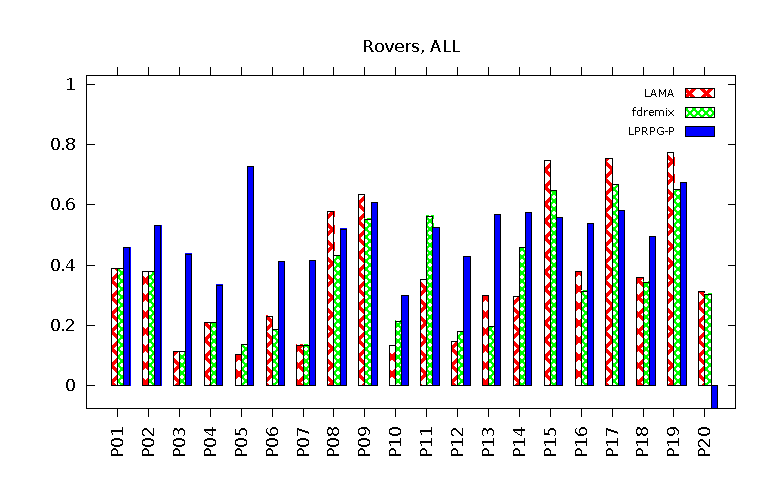
\includegraphics[width=8.5cm]{histogrammi/histogram_rovers_ALL_PERCENTAGE_COST.eps}
\caption{Rovers}
\label{lst:file1}
\end{subfigure}
% &
\\
% TPP ALL HISTOGRAM
\begin{subfigure}[b]{\linewidth}
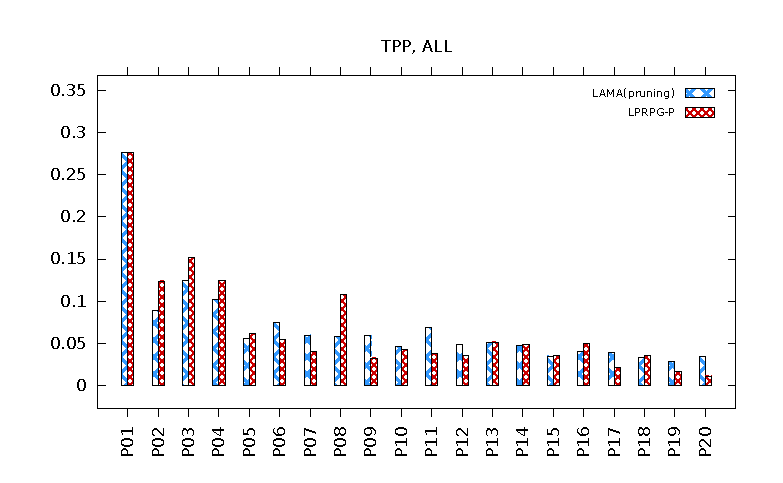
\includegraphics[width=8.5cm]{histogrammi/histogram_tpp_ALL_PERCENTAGE_COST.eps}
\caption{TPP}
\label{lst:file2}
\end{subfigure} \\
% TRUCKS
\begin{subfigure}[b]{\linewidth}
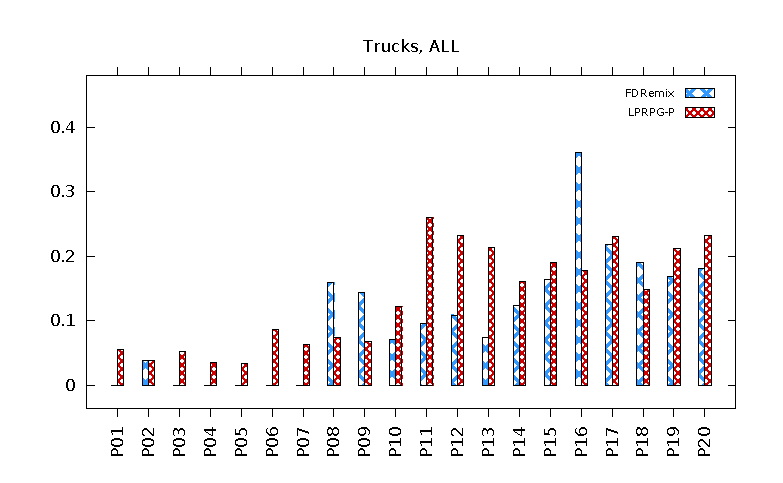
\includegraphics[width=8.5cm]{histogrammi/histogram_trucks_ALL_PERCENTAGE_COST.eps}
\caption{Trucks}
\label{lst:file3}
\end{subfigure}

\end{figure}

\begin{figure}[htb] \ContinuedFloat
% OPENSTACKS
\begin{subfigure}[b]{\linewidth}
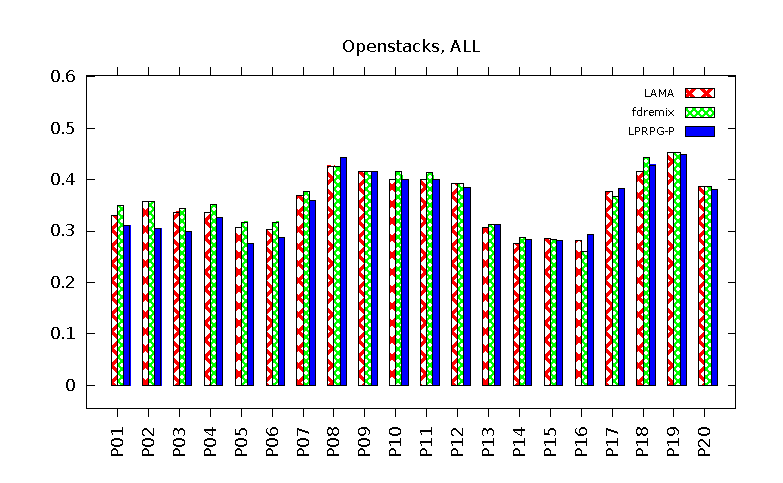
\includegraphics[width=8.5cm]{histogrammi/histogram_openstacks_ALL_PERCENTAGE_COST.eps}
\caption{Openstacks}
\label{lst:file4}
\end{subfigure}
\\
% \end{tabular}
% \begin{tabular}{c}
% STORAGE
\begin{subfigure}[b]{\linewidth}
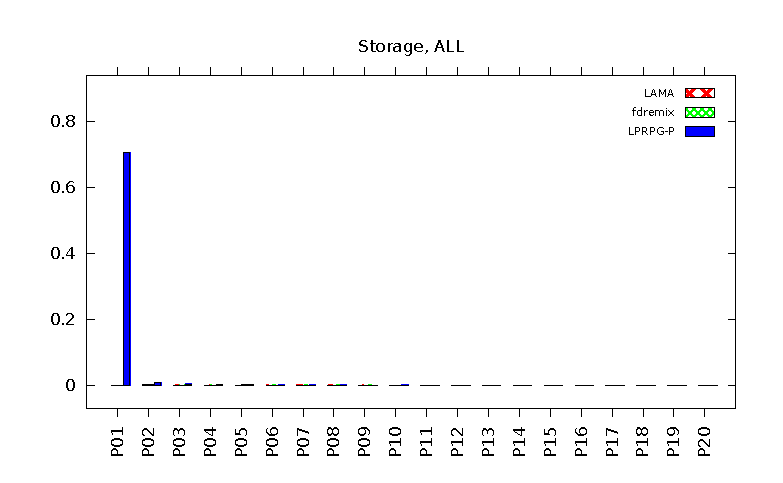
\includegraphics[width=8.5cm]{histogrammi/histogram_preprocessed-storage_ALL_PERCENTAGE_COST.eps}
\caption{Storage}
\label{lst:file5}
\end{subfigure}
\\

% \end{tabular}

% \captionsetup{font=scriptsize}
\caption{Quality Comparison using $\alpha_{\textit{cost}}$ for each domain. Each bar represents the $\alpha_{\textit{cost}}$ of the best plan produced by the considered planner. The negative bar represents an instance which has not been solved or that has no preferences of that kind. From the top to bottom we have provided the results about $\alpha_{\textit{cost}}$ calculated considering each kind of preferences for Rovers, TPP, Trucks, Openstacks and Storage.}
\label{eps:histogram_histograms_ALL_PERCENTAGE_COST}
% \stepcounter{lstlisting}
% \setcounter{figure}{\thetmp}
\end{figure}



% RESTANTI HISTOGRAMMI COMMENTATI

% %%%%%%%%%%%%%%%%%%
% % ROVERS results %
% %%%%%%%%%%%%%%%%%%
% \begin{figure}[H]
% \centering
% \captionof*{table}{Rovers}
% \begin{tabular}{cc}

% \begin{subfigure}{\linewidth}
% 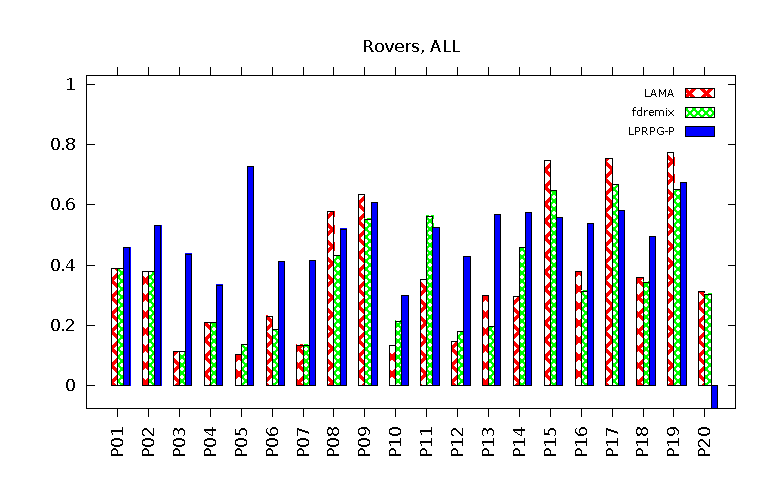
\includegraphics[width=8.5cm]{histogrammi/histogram_rovers_ALL_PERCENTAGE_COST.eps}
% \caption{All}
% \label{lst:file1}
% \end{subfigure}
% &
% \begin{subfigure}{\linewidth}
% 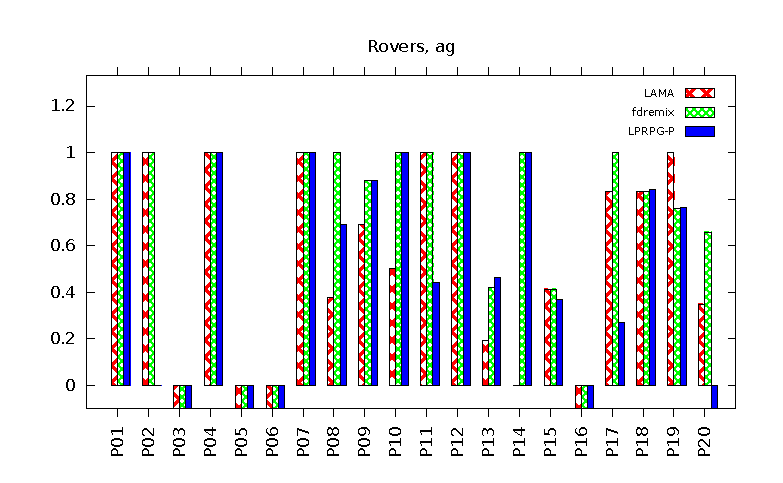
\includegraphics[width=8.5cm]{histogrammi/histogram_rovers_ag_PERCENTAGE_COST.eps}
% \caption{$\mathcal{A}$}
% \label{lst:file2}
% \end{subfigure} \\
% \begin{subfigure}{\linewidth}
% 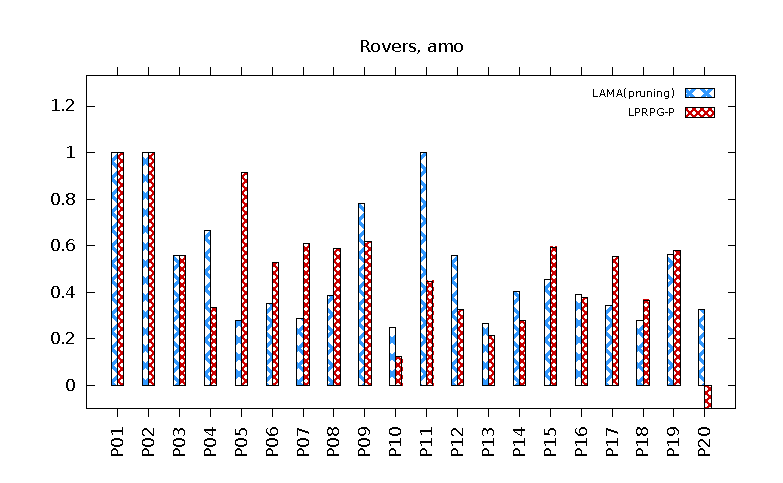
\includegraphics[width=8.5cm]{histogrammi/histogram_rovers_amo_PERCENTAGE_COST.eps}
% \caption{$\mathcal{AO}$}
% \label{lst:file1}
% \end{subfigure}
% &
% \begin{subfigure}{\linewidth}
% 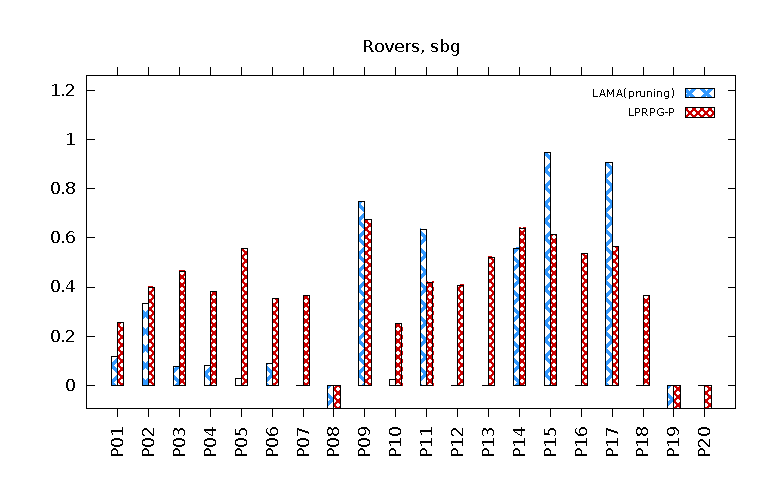
\includegraphics[width=8.5cm]{histogrammi/histogram_rovers_sbg_PERCENTAGE_COST.eps}
% \caption{$\mathcal{SB}$}
% \label{lst:file2}
% \end{subfigure} \\

% \end{tabular}

% \begin{tabular}{c}

% \begin{subfigure}{\linewidth}
% 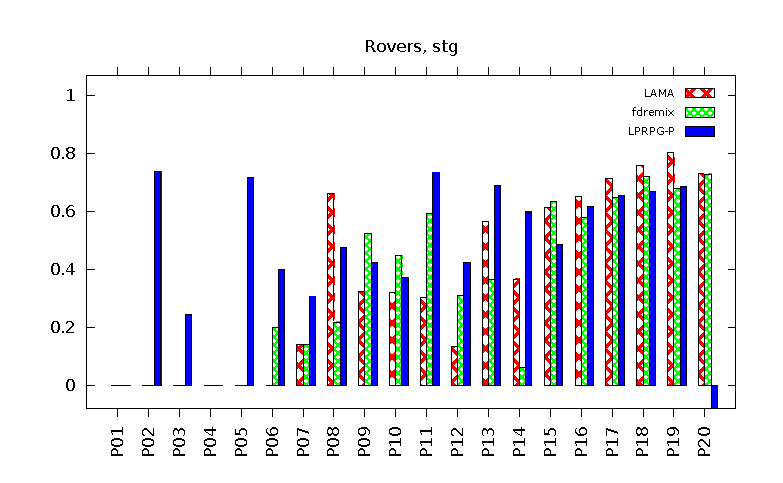
\includegraphics[width=8.5cm]{histogrammi/histogram_rovers_stg_PERCENTAGE_COST.eps}
% \caption{$\mathcal{ST}$}
% \label{lst:file2}
% \end{subfigure} \\

% \end{tabular}


% % \captionsetup{font=scriptsize}
% \caption{Domain: Rovers. Black: LAMA, Grey: IBaCoP2, Light-Grey: LPRPG-P. Each bar represents the $\alpha_{\textit{cost}}$ of the best plan produced by the considered planner. The negative bar represents an instance which has not been solved or that has no preferences of that kind. From left to right we have provided the results about the $\alpha_{\textit{cost}}$ calculated considering each kind of preferences, always, at-most-once, sometime-before and sometime preferences.}
% \label{eps:histogram_histograms_rovers.eps}

% \end{figure}

% %%%%%%%%%%%%%%%
% % TPP results %
% %%%%%%%%%%%%%%%
% \begin{figure}[H]
% \centering

% \begin{tabular}{cc}

% \begin{subfigure}{\linewidth}
% 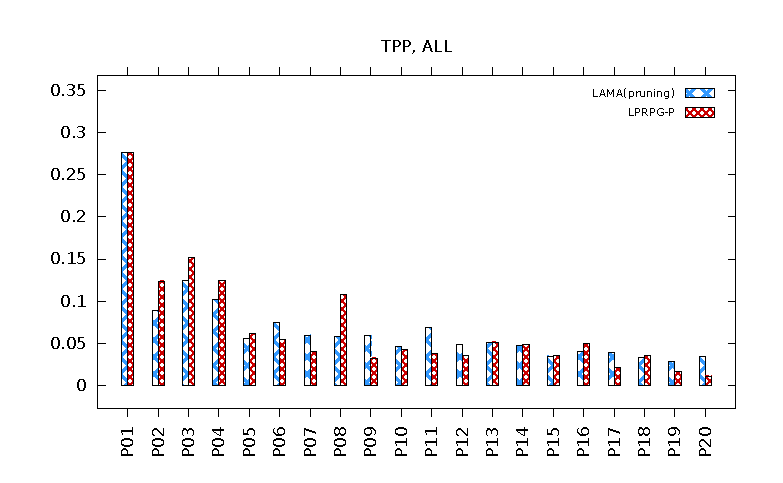
\includegraphics[width=8.5cm]{histogrammi/histogram_tpp_ALL_PERCENTAGE_COST.eps}
% \caption{All}
% \label{lst:tpp:all}
% \end{subfigure}
% &
% \begin{subfigure}{\linewidth}
% 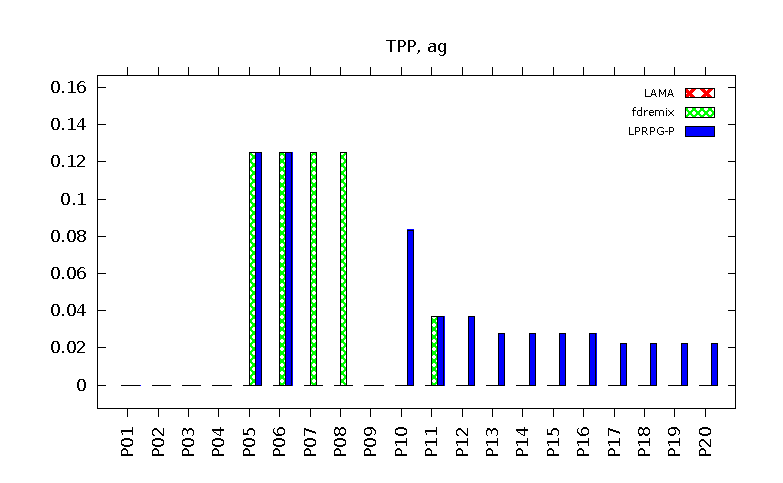
\includegraphics[width=8.5cm]{histogrammi/histogram_tpp_ag_PERCENTAGE_COST.eps}
% \caption{$\mathcal{A}$}
% \label{lst:tpp:ag}
% \end{subfigure} \\
% \begin{subfigure}{\linewidth}
% 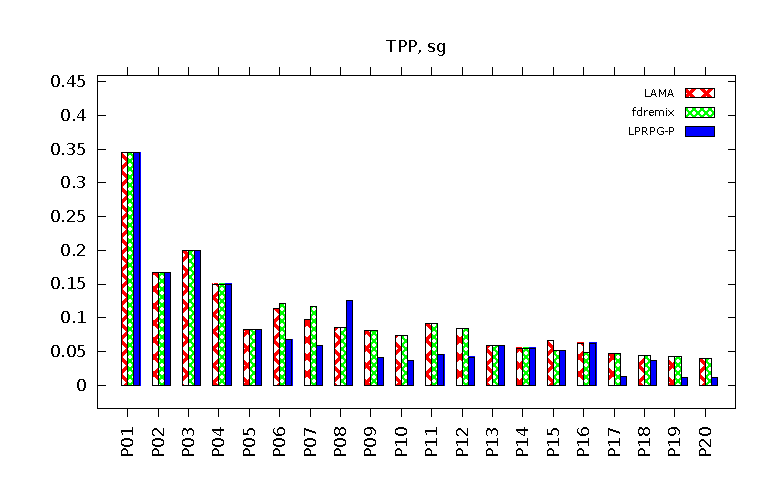
\includegraphics[width=8.5cm]{histogrammi/histogram_tpp_sg_PERCENTAGE_COST.eps}
% \caption{$\mathcal{SG}$}
% \label{lst:tpp:sg}
% \end{subfigure}
% &
% \begin{subfigure}{\linewidth}
% 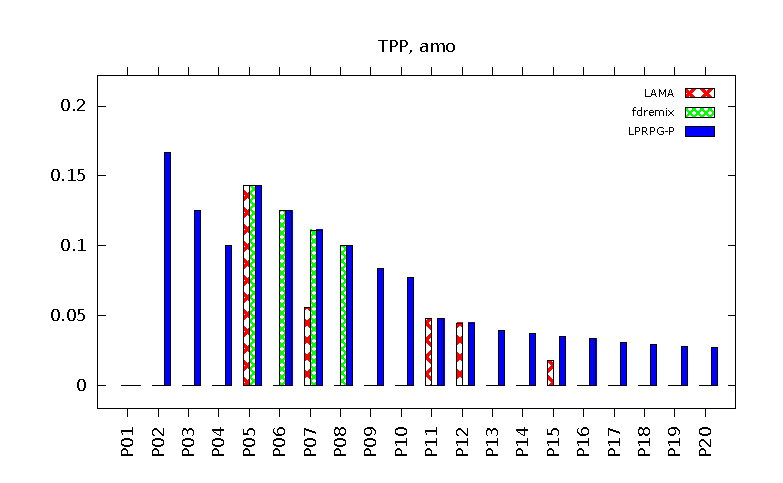
\includegraphics[width=8.5cm]{histogrammi/histogram_tpp_amo_PERCENTAGE_COST.eps}
% \caption{$\mathcal{AO}$}
% \label{lst:tpp:amo}
% \end{subfigure}
% \\
% \begin{subfigure}{\linewidth}
% 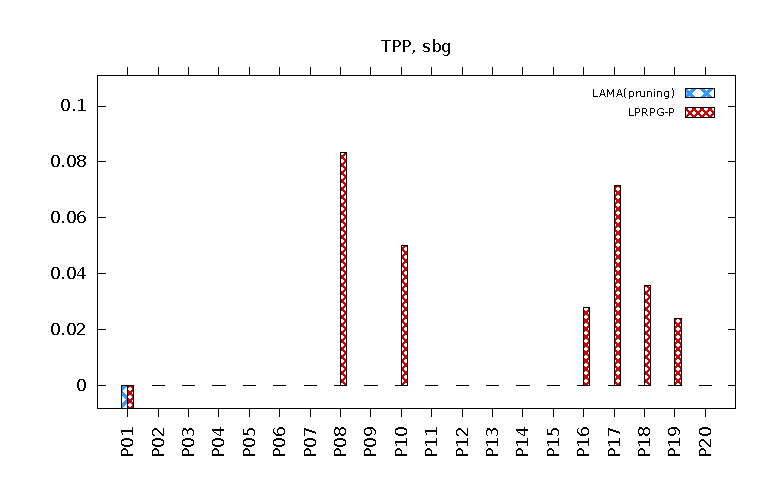
\includegraphics[width=8.5cm]{histogrammi/histogram_tpp_sbg_PERCENTAGE_COST.eps}
% \caption{$\mathcal{SB}$}
% \label{lst:tpp:sbg}
% \end{subfigure}
% &
% \begin{subfigure}{\linewidth}
% 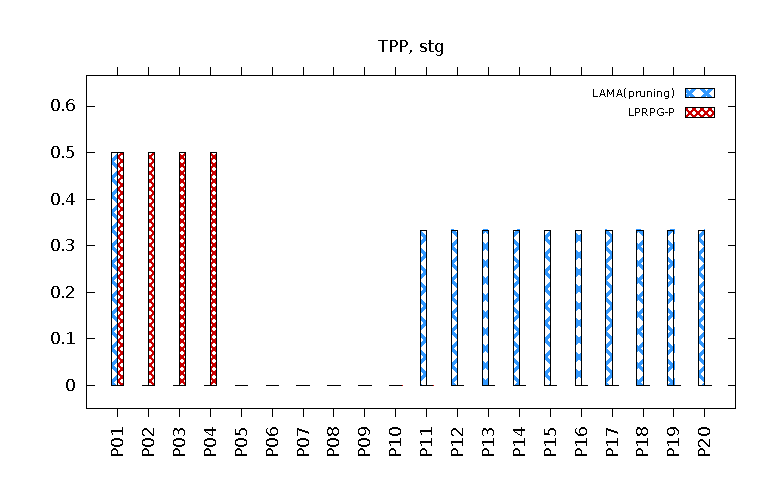
\includegraphics[width=8.5cm]{histogrammi/histogram_tpp_stg_PERCENTAGE_COST.eps}
% \caption{$\mathcal{ST}$}
% \label{lst:file2}
% \end{subfigure}

% \end{tabular}

% % \captionsetup{font=scriptsize}
% \caption{Domain: TPP. Black: LAMA, Grey: IBaCoP2, Light-Grey: LPRPG-P. Each bar represents the $\alpha_{\textit{cost}}$ of the best plan produced by the considered planner. The negative bar represents an instance which has not been solved or that has no preferences of that kind. From left to right we have provided the results about the $\alpha_{\textit{cost}}$ calculated considering each kind of preferences, always, at-end (or soft goals), at-most-once, sometime-before and sometime preferences.}
% \label{eps:histogram_histograms_tpp.eps}

% \end{figure}

% %%%%%%%%%%
% % TRUCKS %
% %%%%%%%%%%
% \begin{figure}[H]
% \centering

% \begin{tabular}{cc}

% % ROVERS ALL HISTOGRAM
% \begin{subfigure}{\linewidth}
% 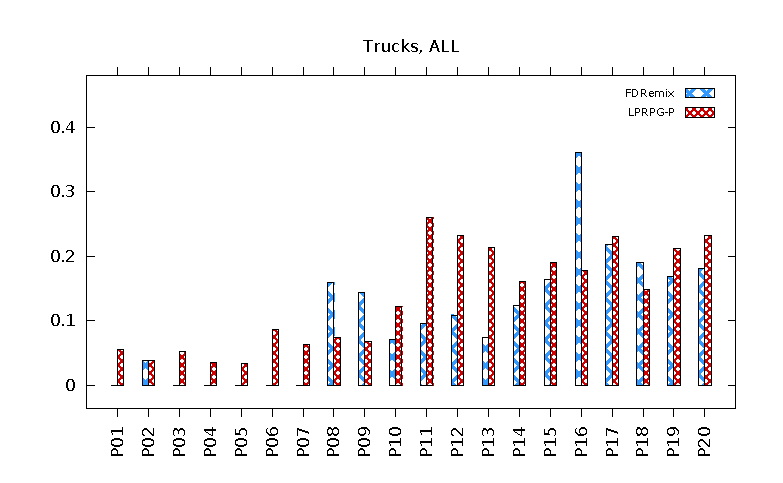
\includegraphics[width=8.5cm]{histogrammi/histogram_trucks_ALL_PERCENTAGE_COST.eps}
% \caption{All}
% \label{lst:file1}
% \end{subfigure}
% &
% % TPP ALL HISTOGRAM
% \begin{subfigure}{\linewidth}
% 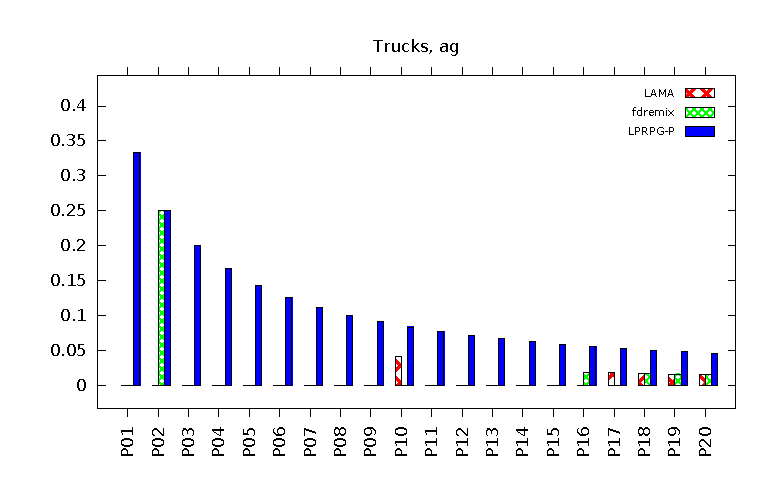
\includegraphics[width=8.5cm]{histogrammi/histogram_trucks_ag_PERCENTAGE_COST.eps}
% \caption{$\mathcal{A}$}
% \label{lst:file2}
% \end{subfigure} \\
% % TRUCKS
% \begin{subfigure}{\linewidth}
% 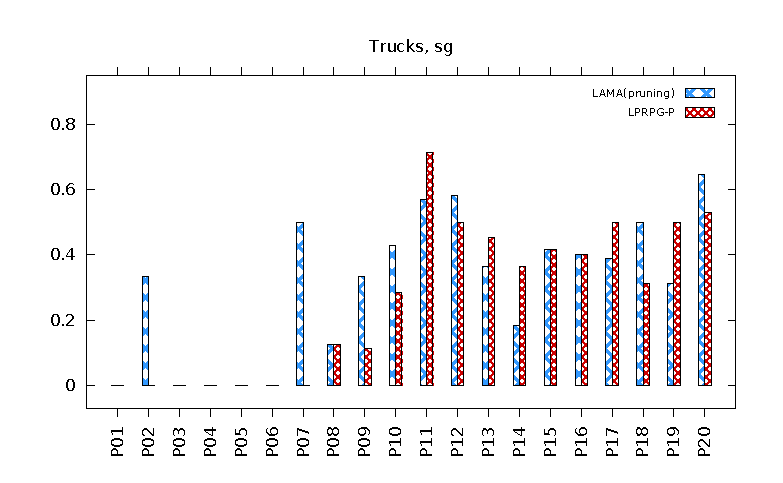
\includegraphics[width=8.5cm]{histogrammi/histogram_trucks_sg_PERCENTAGE_COST.eps}
% \caption{$\mathcal{SG}$}
% \label{lst:file1}
% \end{subfigure}
% &
% % OPENSTACKS
% \begin{subfigure}{\linewidth}
% 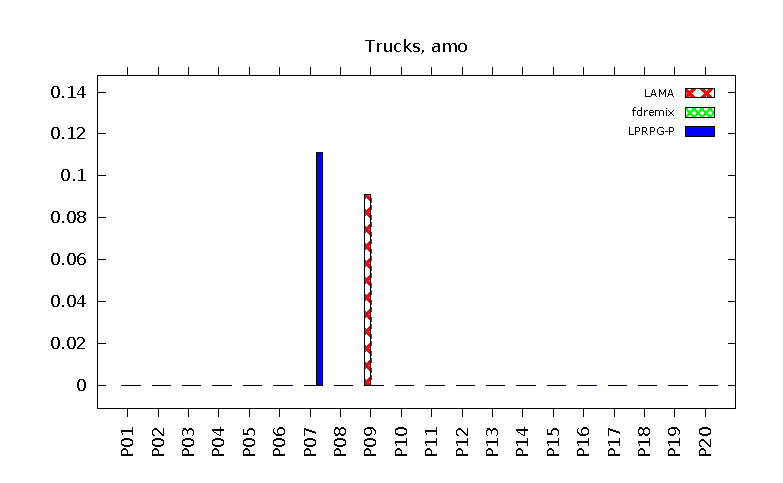
\includegraphics[width=8.5cm]{histogrammi/histogram_trucks_amo_PERCENTAGE_COST.eps}
% \caption{$\mathcal{AO}$}
% \label{lst:file2}
% \end{subfigure} \\

% \end{tabular}

% \begin{tabular}{c}
% % STORAGE
% \begin{subfigure}{\linewidth}
% 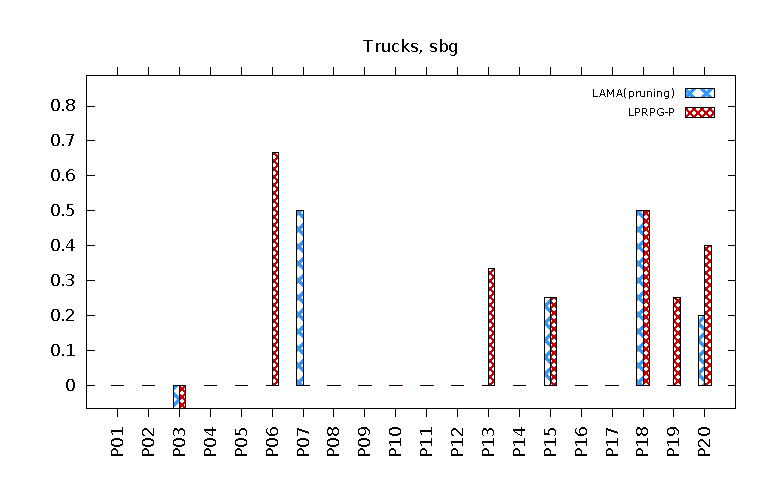
\includegraphics[width=8.5cm]{histogrammi/histogram_trucks_sbg_PERCENTAGE_COST.eps}
% \caption{$\mathcal{SB}$}
% \label{lst:file2}
% \end{subfigure} \\

% \end{tabular}

% % \captionsetup{font=scriptsize}
% \caption{Domain: Trucks. Black: LAMA, Grey: IBaCoP2, Light-Grey: LPRPG-P. Each bar represents the $\alpha_{\textit{cost}}$ of the best plan produced by the considered planner. The negative bar represents an instance which has not been solved or that has no preferences of that kind. From left to right we have provided the results about the $\alpha_{\textit{cost}}$ calculated considering each kind of preferences, always, at-end (or soft goals), at-most-once, sometime-before preferences.}
% \label{eps:histogram_histograms_trucks.eps}

% \end{figure}

% %%%%%%%%%%%%%%
% % OPENSTACKS %
% %%%%%%%%%%%%%%
% \begin{figure}[H]
% \centering

% \begin{tabular}{cc}

% \begin{subfigure}{\linewidth}
% 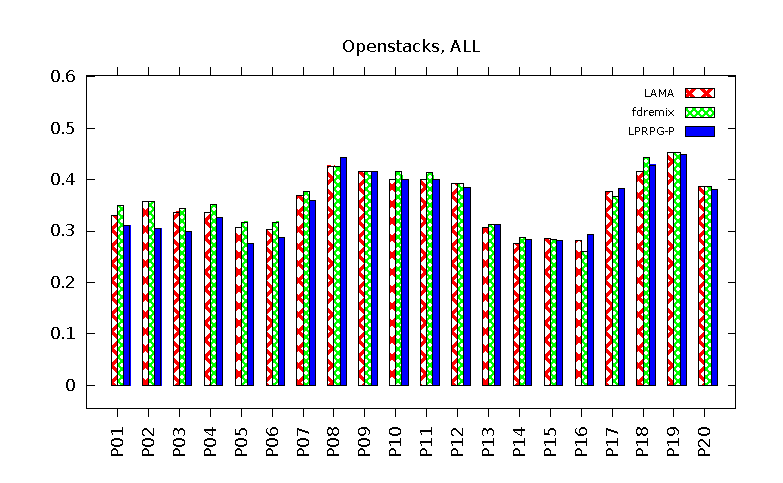
\includegraphics[width=8.5cm]{histogrammi/histogram_openstacks_ALL_PERCENTAGE_COST.eps} 
% \caption{All}
% \label{lst:os:all}
% \end{subfigure}
% &

% \begin{subfigure}{\linewidth}
% 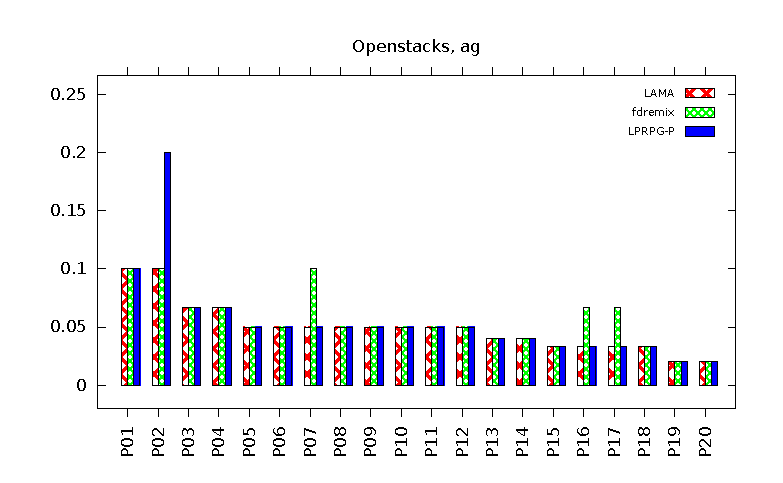
\includegraphics[width=8.5cm]{histogrammi/histogram_openstacks_ag_PERCENTAGE_COST.eps}
% \caption{$\mathcal{A}$}
% \label{lst:os:ag}
% \end{subfigure}
% \\

% \end{tabular}

% \begin{tabular}{c}

% \begin{subfigure}{\linewidth}
% 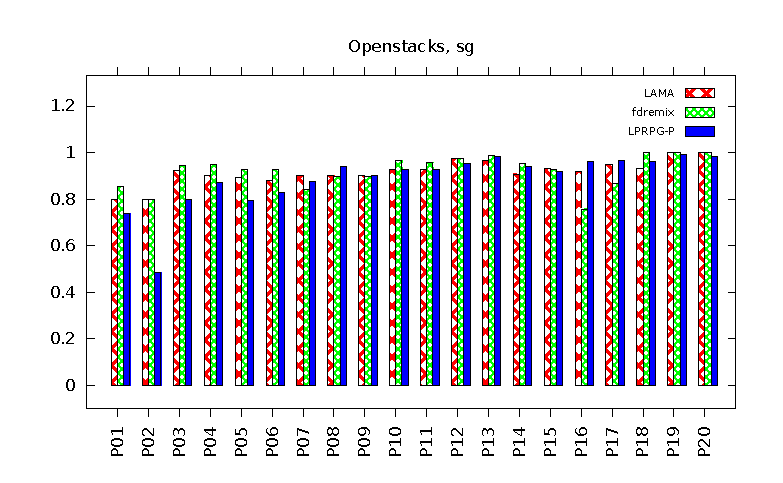
\includegraphics[width=8.5cm]{histogrammi/histogram_openstacks_sg_PERCENTAGE_COST.eps}
% \caption{$\mathcal{SG}$}
% \label{lst:os:sg}
% \end{subfigure}

% \end{tabular}

% % \captionsetup{font=scriptsize}
% \caption{Domain: Openstacks. Black: LAMA, Grey: IBaCoP2, Light-Grey: LPRPG-P. Each bar represents the $\alpha_{\textit{cost}}$ of the best plan produced by the considered planner. The negative bar represents an instance which has not been solved or that has no preferences of that kind. From left to right we have provided the results about the $\alpha_{\textit{cost}}$ calculated considering each kind of preferences, always and at end (or soft goals) preferences.}
% \label{eps:histogram_histograms_openstacks.eps}

% \end{figure}


% %%%%%%%%%%%%%%%%%%%
% % STORAGE results %
% %%%%%%%%%%%%%%%%%%%
% \begin{figure}[H]
% \centering

% \begin{tabular}{cc}

% \begin{subfigure}{\linewidth}
% 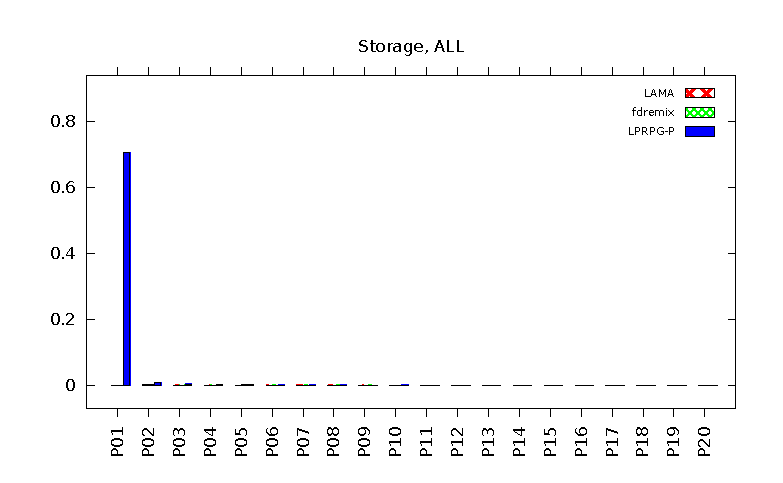
\includegraphics[width=8.5cm]{histogrammi/histogram_preprocessed-storage_ALL_PERCENTAGE_COST.eps}
% \caption{All}
% \label{lst:file1}
% \end{subfigure}
% &
% \begin{subfigure}{\linewidth}
% 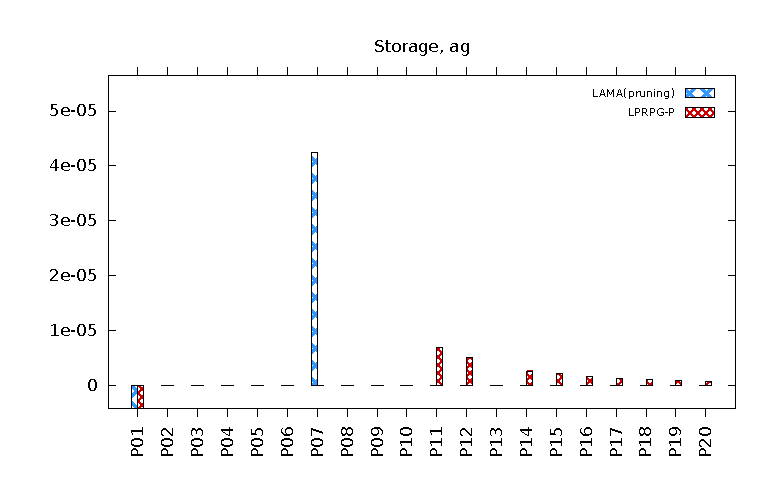
\includegraphics[width=8.5cm]{histogrammi/histogram_preprocessed-storage_ag_PERCENTAGE_COST.eps}
% \caption{$\mathcal{A}$}
% \label{lst:file2}
% \end{subfigure} \\
% \begin{subfigure}{\linewidth}
% 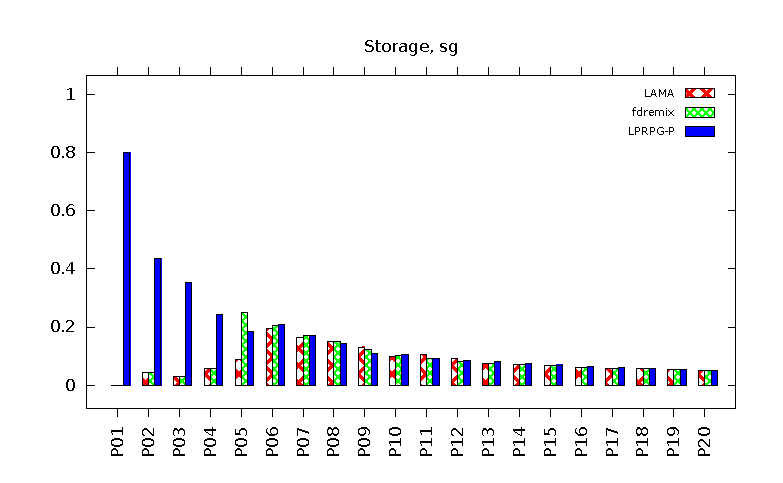
\includegraphics[width=8.5cm]{histogrammi/histogram_preprocessed-storage_sg_PERCENTAGE_COST.eps}
% \caption{$\mathcal{SG}$}
% \label{lst:file1}
% \end{subfigure}
% &
% \begin{subfigure}{\linewidth}
% 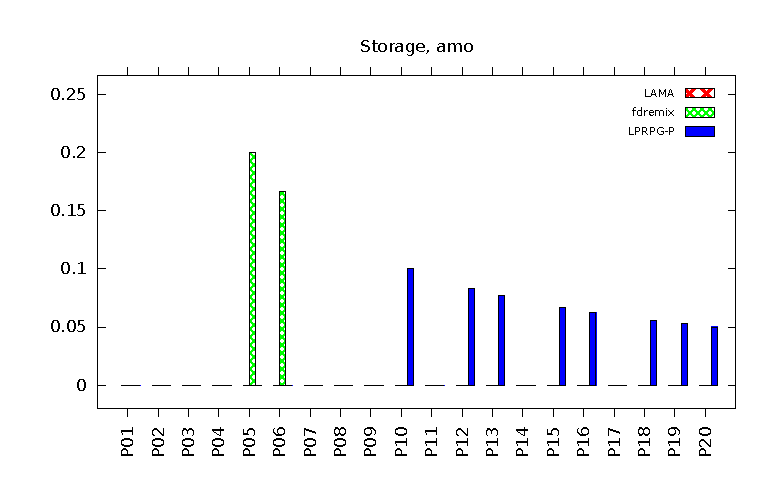
\includegraphics[width=8.5cm]{histogrammi/histogram_preprocessed-storage_amo_PERCENTAGE_COST.eps}
% \caption{$\mathcal{AO}$}
% \label{lst:file2}
% \end{subfigure}
% \\
% \begin{subfigure}{\linewidth}
% 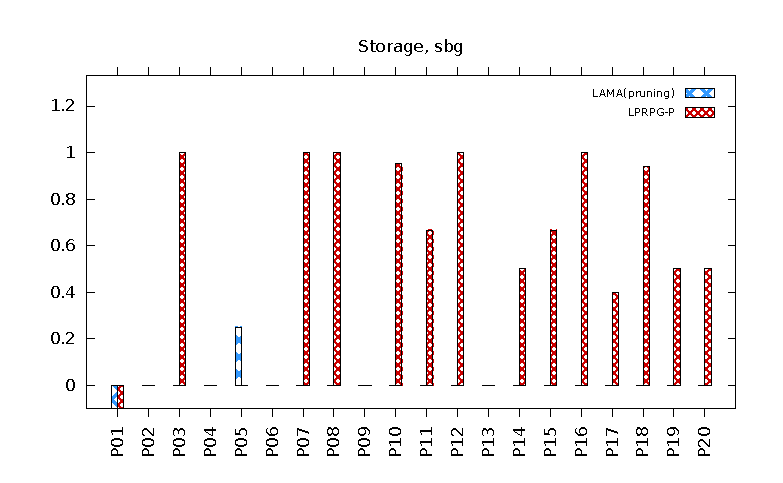
\includegraphics[width=8.5cm]{histogrammi/histogram_preprocessed-storage_sbg_PERCENTAGE_COST.eps}
% \caption{$\mathcal{SB}$}
% \label{lst:file2}
% \end{subfigure}
% &
% \begin{subfigure}{\linewidth}
% 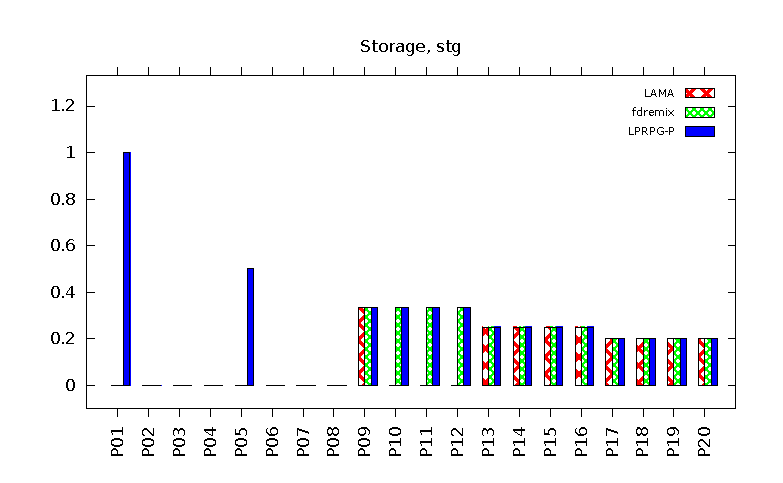
\includegraphics[width=8.5cm]{histogrammi/histogram_preprocessed-storage_stg_PERCENTAGE_COST.eps}
% \caption{$\mathcal{ST}$}
% \label{lst:file2}
% \end{subfigure}

% \end{tabular}


% % \captionsetup{font=scriptsize}
% \caption{Domain: Storage. Black: LAMA, Grey: IBaCoP2, Light-Grey: LPRPG-P. Each bar represents the $\alpha_{\textit{cost}}$ of the best plan produced by the considered planner. The negative bar represents an instance which has not been solved or that has no preferences of that kind. From left to right we have provided the results about the $\alpha_{\textit{cost}}$ calculated considering each kind of preferences, always, at-end (or soft goals), at-most-once, sometime-before and sometime preferences.}
% \label{eps:histogram_histograms_storage.eps}

% \end{figure}


\subsection{Optimal Planning Results}

Similarly to what to what has been done in \cite{nebel2018}, we have tested our scheme
using some admissible heuristics which are $h^\text{blind}$, $h^\text{max}$ an $h^{\text{M\&S}}$ which guarantee us the optimality of the solution found. Starting from the IPC5 domains, we generated
simpler instances by randomly sampling subsets of the soft trajectory constraints. Starting
from each instance we have generated five new instances with 1\%, 5\%, 10\%, 20\% and 40\% of
the (grounded) soft trajectory constraints while the hard goals have remained unchanged.

Since we do not have the instances that have been used in the aforementioned paper,
we have generated, for each percentage of sampling preferences (excpet for 100 \%), five sampled
instances in order to average the obtained results. The results about 
this experiment are shown Table \ref{coverage_admissible_heuristics}. The results
inherent to Openstacks have been excluded because it was not possible to find optimal
plans even for the simplest instances.


\begin{table}[]
\scriptsize
\centering
\begin{tabular}{|c|c|c|c|}
\hline 
Domain & $h^{\text{blind}}$ & $h^{\text{max}}$ & $h^{\text{m\&s}}$\\ \hline 
Storage & 49.0& 41.0& 23.0\\ \hline 
Rovers & 23.0& 23.0& 23.0\\ \hline 
TPP-p & 36.0& 33.0& 35.0\\ \hline 
Trucks & 23.0& 28.0& 23.0\\ \hline 
TOTAL & 33.0& 31.0& 26.0\\ \hline 

\end{tabular}
\caption{Coverage of our compilation scheme on the IPC5 benchmarks set with
additional instances with random sampled soft-trajectory constraints, A*
search for optimal solution.}\label{coverage_admissible_heuristics}
\end{table}


\section{Conclusions}



\bibliographystyle{plain}
\bibliography{biblio.bib}
\end{document}
